\documentclass[twoside]{book}

% Packages required by doxygen
\usepackage{fixltx2e}
\usepackage{calc}
\usepackage{doxygen}
\usepackage[export]{adjustbox} % also loads graphicx
\usepackage{graphicx}
\usepackage[utf8]{inputenc}
\usepackage{makeidx}
\usepackage{multicol}
\usepackage{multirow}
\PassOptionsToPackage{warn}{textcomp}
\usepackage{textcomp}
\usepackage[nointegrals]{wasysym}
\usepackage[table]{xcolor}

% Font selection
\usepackage[T1]{fontenc}
\usepackage[scaled=.90]{helvet}
\usepackage{courier}
\usepackage{amssymb}
\usepackage{sectsty}
\renewcommand{\familydefault}{\sfdefault}
\allsectionsfont{%
  \fontseries{bc}\selectfont%
  \color{darkgray}%
}
\renewcommand{\DoxyLabelFont}{%
  \fontseries{bc}\selectfont%
  \color{darkgray}%
}
\newcommand{\+}{\discretionary{\mbox{\scriptsize$\hookleftarrow$}}{}{}}

% Page & text layout
\usepackage{geometry}
\geometry{%
  a4paper,%
  top=2.5cm,%
  bottom=2.5cm,%
  left=2.5cm,%
  right=2.5cm%
}
\tolerance=750
\hfuzz=15pt
\hbadness=750
\setlength{\emergencystretch}{15pt}
\setlength{\parindent}{0cm}
\setlength{\parskip}{3ex plus 2ex minus 2ex}
\makeatletter
\renewcommand{\paragraph}{%
  \@startsection{paragraph}{4}{0ex}{-1.0ex}{1.0ex}{%
    \normalfont\normalsize\bfseries\SS@parafont%
  }%
}
\renewcommand{\subparagraph}{%
  \@startsection{subparagraph}{5}{0ex}{-1.0ex}{1.0ex}{%
    \normalfont\normalsize\bfseries\SS@subparafont%
  }%
}
\makeatother

% Headers & footers
\usepackage{fancyhdr}
\pagestyle{fancyplain}
\fancyhead[LE]{\fancyplain{}{\bfseries\thepage}}
\fancyhead[CE]{\fancyplain{}{}}
\fancyhead[RE]{\fancyplain{}{\bfseries\leftmark}}
\fancyhead[LO]{\fancyplain{}{\bfseries\rightmark}}
\fancyhead[CO]{\fancyplain{}{}}
\fancyhead[RO]{\fancyplain{}{\bfseries\thepage}}
\fancyfoot[LE]{\fancyplain{}{}}
\fancyfoot[CE]{\fancyplain{}{}}
\fancyfoot[RE]{\fancyplain{}{\bfseries\scriptsize Generated by Doxygen }}
\fancyfoot[LO]{\fancyplain{}{\bfseries\scriptsize Generated by Doxygen }}
\fancyfoot[CO]{\fancyplain{}{}}
\fancyfoot[RO]{\fancyplain{}{}}
\renewcommand{\footrulewidth}{0.4pt}
\renewcommand{\chaptermark}[1]{%
  \markboth{#1}{}%
}
\renewcommand{\sectionmark}[1]{%
  \markright{\thesection\ #1}%
}

% Indices & bibliography
\usepackage{natbib}
\usepackage[titles]{tocloft}
\setcounter{tocdepth}{3}
\setcounter{secnumdepth}{5}
\makeindex

% Hyperlinks (required, but should be loaded last)
\usepackage{ifpdf}
\ifpdf
  \usepackage[pdftex,pagebackref=true]{hyperref}
\else
  \usepackage[ps2pdf,pagebackref=true]{hyperref}
\fi
\hypersetup{%
  colorlinks=true,%
  linkcolor=blue,%
  citecolor=blue,%
  unicode%
}

% Custom commands
\newcommand{\clearemptydoublepage}{%
  \newpage{\pagestyle{empty}\cleardoublepage}%
}

\usepackage{caption}
\captionsetup{labelsep=space,justification=centering,font={bf},singlelinecheck=off,skip=4pt,position=top}

%===== C O N T E N T S =====

\begin{document}

% Titlepage & ToC
\hypersetup{pageanchor=false,
             bookmarksnumbered=true,
             pdfencoding=unicode
            }
\pagenumbering{alph}
\begin{titlepage}
\vspace*{7cm}
\begin{center}%
{\Large My Project }\\
\vspace*{1cm}
{\large Generated by Doxygen 1.8.14}\\
\end{center}
\end{titlepage}
\clearemptydoublepage
\pagenumbering{roman}
\tableofcontents
\clearemptydoublepage
\pagenumbering{arabic}
\hypersetup{pageanchor=true}

%--- Begin generated contents ---
\chapter{R\+E\+A\+D\+ME}
\label{md__r_e_a_d_m_e}
\Hypertarget{md__r_e_a_d_m_e}
Hannes project

\href{https://gitlab.mpikg.mpg.de/baukmann/hannesProjekt/blob/master/html/index.html}{\tt Documentation} 
\chapter{Namespace Index}
\section{Namespace List}
Here is a list of all documented namespaces with brief descriptions\+:\begin{DoxyCompactList}
\item\contentsline{section}{\mbox{\hyperlink{namespace_hannes_o_o_p_project}{Hannes\+O\+O\+P\+Project}} \\*Description of this project }{\pageref{namespace_hannes_o_o_p_project}}{}
\end{DoxyCompactList}

\chapter{Hierarchical Index}
\section{Class Hierarchy}
This inheritance list is sorted roughly, but not completely, alphabetically\+:\begin{DoxyCompactList}
\item \contentsline{section}{O\+O\+P.\+Analysis}{\pageref{class_o_o_p_1_1_analysis}}{}
\item \contentsline{section}{O\+O\+P\+\_\+np\+Array.\+Analysis}{\pageref{class_o_o_p__np_array_1_1_analysis}}{}
\item \contentsline{section}{O\+O\+P\+\_\+np\+Array.\+Builder}{\pageref{class_o_o_p__np_array_1_1_builder}}{}
\item \contentsline{section}{O\+O\+P.\+Builder}{\pageref{class_o_o_p_1_1_builder}}{}
\item \contentsline{section}{O\+O\+P\+\_\+np\+Array.\+Cytokine}{\pageref{class_o_o_p__np_array_1_1_cytokine}}{}
\item \contentsline{section}{O\+O\+P.\+Cytokine}{\pageref{class_o_o_p_1_1_cytokine}}{}
\item \contentsline{section}{O\+O\+P.\+Glycan}{\pageref{class_o_o_p_1_1_glycan}}{}
\item \contentsline{section}{O\+O\+P\+\_\+np\+Array.\+Glycan}{\pageref{class_o_o_p__np_array_1_1_glycan}}{}
\item \contentsline{section}{O\+O\+P.\+Lectin}{\pageref{class_o_o_p_1_1_lectin}}{}
\item \contentsline{section}{O\+O\+P\+\_\+np\+Array.\+Lectin}{\pageref{class_o_o_p__np_array_1_1_lectin}}{}
\item \contentsline{section}{O\+O\+P.\+Simulation}{\pageref{class_o_o_p_1_1_simulation}}{}
\item \contentsline{section}{O\+O\+P\+\_\+np\+Array.\+Simulation}{\pageref{class_o_o_p__np_array_1_1_simulation}}{}
\item \contentsline{section}{O\+O\+P.\+Sphere}{\pageref{class_o_o_p_1_1_sphere}}{}
\begin{DoxyCompactList}
\item \contentsline{section}{O\+O\+P.\+Bead}{\pageref{class_o_o_p_1_1_bead}}{}
\item \contentsline{section}{O\+O\+P.\+Decoder\+Cell}{\pageref{class_o_o_p_1_1_decoder_cell}}{}
\end{DoxyCompactList}
\item \contentsline{section}{O\+O\+P\+\_\+np\+Array.\+Sphere}{\pageref{class_o_o_p__np_array_1_1_sphere}}{}
\begin{DoxyCompactList}
\item \contentsline{section}{O\+O\+P\+\_\+np\+Array.\+Bead}{\pageref{class_o_o_p__np_array_1_1_bead}}{}
\item \contentsline{section}{O\+O\+P\+\_\+np\+Array.\+Decoder\+Cell}{\pageref{class_o_o_p__np_array_1_1_decoder_cell}}{}
\end{DoxyCompactList}
\item \contentsline{section}{O\+O\+P\+\_\+np\+Array.\+Well}{\pageref{class_o_o_p__np_array_1_1_well}}{}
\begin{DoxyCompactList}
\item \contentsline{section}{O\+O\+P\+\_\+np\+Array.\+Well\+\_\+list}{\pageref{class_o_o_p__np_array_1_1_well__list}}{}
\item \contentsline{section}{O\+O\+P\+\_\+np\+Array.\+Well\+\_\+np\+Array}{\pageref{class_o_o_p__np_array_1_1_well__np_array}}{}
\end{DoxyCompactList}
\item \contentsline{section}{O\+O\+P.\+Well}{\pageref{class_o_o_p_1_1_well}}{}
\end{DoxyCompactList}

\chapter{Class Index}
\section{Class List}
Here are the classes, structs, unions and interfaces with brief descriptions\+:\begin{DoxyCompactList}
\item\contentsline{section}{\mbox{\hyperlink{class_o_o_p_1_1_cell}{O\+O\+P.\+Cell}} \\*Dokumentation for class \mbox{\hyperlink{class_o_o_p_1_1_cell}{Cell}} }{\pageref{class_o_o_p_1_1_cell}}{}
\item\contentsline{section}{\mbox{\hyperlink{class_o_o_p_1_1_decoder_cell}{O\+O\+P.\+Decoder\+Cell}} }{\pageref{class_o_o_p_1_1_decoder_cell}}{}
\item\contentsline{section}{\mbox{\hyperlink{class_o_o_p_1_1_encoder_cell}{O\+O\+P.\+Encoder\+Cell}} }{\pageref{class_o_o_p_1_1_encoder_cell}}{}
\item\contentsline{section}{\mbox{\hyperlink{class_o_o_p_1_1_glycan}{O\+O\+P.\+Glycan}} }{\pageref{class_o_o_p_1_1_glycan}}{}
\item\contentsline{section}{\mbox{\hyperlink{class_o_o_p_1_1_lectin}{O\+O\+P.\+Lectin}} }{\pageref{class_o_o_p_1_1_lectin}}{}
\item\contentsline{section}{\mbox{\hyperlink{classprototype_1_1_object_factory}{prototype.\+Object\+Factory}} }{\pageref{classprototype_1_1_object_factory}}{}
\item\contentsline{section}{\mbox{\hyperlink{classprototype_1_1_prototype}{prototype.\+Prototype}} }{\pageref{classprototype_1_1_prototype}}{}
\item\contentsline{section}{\mbox{\hyperlink{classprototype_1_1_type1}{prototype.\+Type1}} }{\pageref{classprototype_1_1_type1}}{}
\item\contentsline{section}{\mbox{\hyperlink{classprototype_1_1_type2}{prototype.\+Type2}} }{\pageref{classprototype_1_1_type2}}{}
\end{DoxyCompactList}

\chapter{Namespace Documentation}
\hypertarget{namespace_hannes_o_o_p_project}{}\section{Hannes\+O\+O\+P\+Project Namespace Reference}
\label{namespace_hannes_o_o_p_project}\index{Hannes\+O\+O\+P\+Project@{Hannes\+O\+O\+P\+Project}}


Description of this project.  




\subsection{Detailed Description}
Description of this project. 

\subsection*{Ueberschift! }
\chapter{Class Documentation}
\hypertarget{class_o_o_p_1_1_analysis}{}\section{O\+O\+P.\+Analysis Class Reference}
\label{class_o_o_p_1_1_analysis}\index{O\+O\+P.\+Analysis@{O\+O\+P.\+Analysis}}
\subsection*{Public Member Functions}
\begin{DoxyCompactItemize}
\item 
\mbox{\Hypertarget{class_o_o_p_1_1_analysis_ab4b7c43065313c288381613d4f8aef98}\label{class_o_o_p_1_1_analysis_ab4b7c43065313c288381613d4f8aef98}} 
def {\bfseries \+\_\+\+\_\+init\+\_\+\+\_\+} (self)
\item 
\mbox{\Hypertarget{class_o_o_p_1_1_analysis_ac546b71a8d77db12fdc51bc082663e05}\label{class_o_o_p_1_1_analysis_ac546b71a8d77db12fdc51bc082663e05}} 
def {\bfseries count\+Cytokines} (self, simulation\+Results)
\item 
\mbox{\Hypertarget{class_o_o_p_1_1_analysis_af92b055dfa67cb7e686755f7c41674df}\label{class_o_o_p_1_1_analysis_af92b055dfa67cb7e686755f7c41674df}} 
def {\bfseries plot\+Cytokines} (self, simulation\+Results)
\end{DoxyCompactItemize}
\subsection*{Public Attributes}
\begin{DoxyCompactItemize}
\item 
\mbox{\Hypertarget{class_o_o_p_1_1_analysis_a6081436f5f7f9cffc37e7363baee1f4d}\label{class_o_o_p_1_1_analysis_a6081436f5f7f9cffc37e7363baee1f4d}} 
{\bfseries cytokine\+Amount}
\item 
\mbox{\Hypertarget{class_o_o_p_1_1_analysis_aeaa2243b8bbc7c25dfd075fee3df26af}\label{class_o_o_p_1_1_analysis_aeaa2243b8bbc7c25dfd075fee3df26af}} 
{\bfseries cytokine\+Names}
\end{DoxyCompactItemize}


The documentation for this class was generated from the following file\+:\begin{DoxyCompactItemize}
\item 
O\+O\+P.\+py\end{DoxyCompactItemize}

\hypertarget{class_o_o_p_1_1_bead}{}\section{O\+O\+P.\+Bead Class Reference}
\label{class_o_o_p_1_1_bead}\index{O\+O\+P.\+Bead@{O\+O\+P.\+Bead}}
Inheritance diagram for O\+O\+P.\+Bead\+:\begin{figure}[H]
\begin{center}
\leavevmode
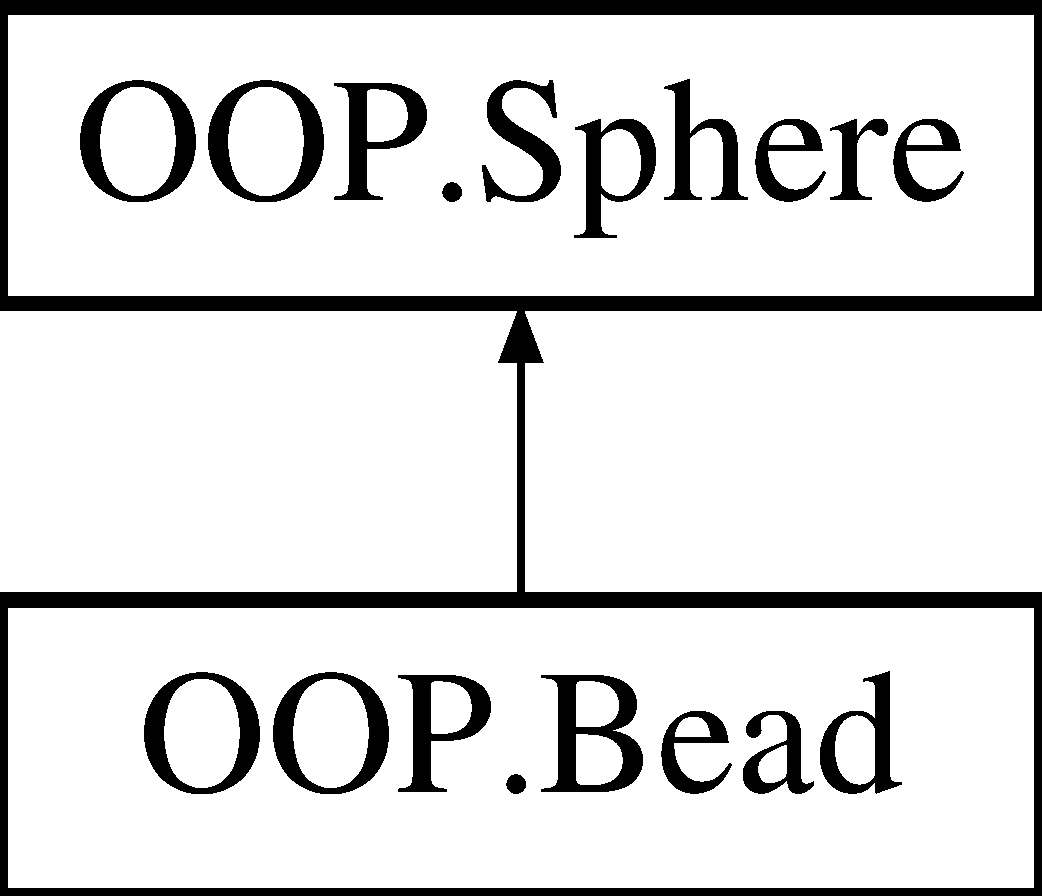
\includegraphics[height=2.000000cm]{class_o_o_p_1_1_bead}
\end{center}
\end{figure}
\subsection*{Public Member Functions}
\begin{DoxyCompactItemize}
\item 
\mbox{\Hypertarget{class_o_o_p_1_1_bead_a0bbaef493483785c91a9d65119cf03f7}\label{class_o_o_p_1_1_bead_a0bbaef493483785c91a9d65119cf03f7}} 
def {\bfseries \+\_\+\+\_\+init\+\_\+\+\_\+} (self, args)
\item 
\mbox{\Hypertarget{class_o_o_p_1_1_bead_a5c3fdb6f49fa45d5484e7fa1547e11d9}\label{class_o_o_p_1_1_bead_a5c3fdb6f49fa45d5484e7fa1547e11d9}} 
def {\bfseries attach\+Glycans} (self, glycan\+\_\+names\+\_\+list, glycan\+\_\+types\+\_\+list, density\+\_\+percentage)
\end{DoxyCompactItemize}
\subsection*{Public Attributes}
\begin{DoxyCompactItemize}
\item 
\mbox{\Hypertarget{class_o_o_p_1_1_bead_a6077018c22bee0df53ac3f034a5cc43e}\label{class_o_o_p_1_1_bead_a6077018c22bee0df53ac3f034a5cc43e}} 
{\bfseries glycan\+\_\+density}
\item 
\mbox{\Hypertarget{class_o_o_p_1_1_bead_a889f4d823c56c1a5ef77f720167de381}\label{class_o_o_p_1_1_bead_a889f4d823c56c1a5ef77f720167de381}} 
{\bfseries glycan}
\end{DoxyCompactItemize}


The documentation for this class was generated from the following file\+:\begin{DoxyCompactItemize}
\item 
O\+O\+P.\+py\end{DoxyCompactItemize}

\hypertarget{class_o_o_p_1_1_builder}{}\section{O\+O\+P.\+Builder Class Reference}
\label{class_o_o_p_1_1_builder}\index{O\+O\+P.\+Builder@{O\+O\+P.\+Builder}}
\subsection*{Public Member Functions}
\begin{DoxyCompactItemize}
\item 
\mbox{\Hypertarget{class_o_o_p_1_1_builder_a411b856c6a67394b5b5bb22a1d842084}\label{class_o_o_p_1_1_builder_a411b856c6a67394b5b5bb22a1d842084}} 
def {\bfseries \+\_\+\+\_\+init\+\_\+\+\_\+} (self, x, y, z)
\item 
\mbox{\Hypertarget{class_o_o_p_1_1_builder_a0eea0de9ec4e52ee06655026a639ccda}\label{class_o_o_p_1_1_builder_a0eea0de9ec4e52ee06655026a639ccda}} 
def {\bfseries build\+Well} (self)
\item 
\mbox{\Hypertarget{class_o_o_p_1_1_builder_a3d3b6a5868e3ff78e55f2f56643a093c}\label{class_o_o_p_1_1_builder_a3d3b6a5868e3ff78e55f2f56643a093c}} 
def {\bfseries build\+Bead} (self, ID, glyan\+\_\+name\+\_\+string, glycan\+\_\+type\+\_\+string, density\+\_\+percentage)
\item 
\mbox{\Hypertarget{class_o_o_p_1_1_builder_aee394a36797057d3062e8cc00ae0bf62}\label{class_o_o_p_1_1_builder_aee394a36797057d3062e8cc00ae0bf62}} 
def {\bfseries build\+Decoder\+Cell} (self, ID, lectin\+\_\+name\+\_\+string, density\+\_\+percentage)
\end{DoxyCompactItemize}
\subsection*{Public Attributes}
\begin{DoxyCompactItemize}
\item 
\mbox{\Hypertarget{class_o_o_p_1_1_builder_a1b32d7d61a14024383c1653ce6395929}\label{class_o_o_p_1_1_builder_a1b32d7d61a14024383c1653ce6395929}} 
{\bfseries x}
\item 
\mbox{\Hypertarget{class_o_o_p_1_1_builder_af0f4e96f7f484650e51fdb8c85245686}\label{class_o_o_p_1_1_builder_af0f4e96f7f484650e51fdb8c85245686}} 
{\bfseries y}
\item 
\mbox{\Hypertarget{class_o_o_p_1_1_builder_aaa4ad6ace7fd3ca021dc3aec3e13244f}\label{class_o_o_p_1_1_builder_aaa4ad6ace7fd3ca021dc3aec3e13244f}} 
{\bfseries z}
\item 
\mbox{\Hypertarget{class_o_o_p_1_1_builder_ad64e4b7688e8ff3fcc91bf6b097fe819}\label{class_o_o_p_1_1_builder_ad64e4b7688e8ff3fcc91bf6b097fe819}} 
{\bfseries well}
\end{DoxyCompactItemize}


The documentation for this class was generated from the following file\+:\begin{DoxyCompactItemize}
\item 
O\+O\+P.\+py\end{DoxyCompactItemize}

\hypertarget{class_o_o_p_1_1_cytokine}{}\section{O\+O\+P.\+Cytokine Class Reference}
\label{class_o_o_p_1_1_cytokine}\index{O\+O\+P.\+Cytokine@{O\+O\+P.\+Cytokine}}
\subsection*{Public Member Functions}
\begin{DoxyCompactItemize}
\item 
\mbox{\Hypertarget{class_o_o_p_1_1_cytokine_ac53d9c48326010876cfdd9bce36ada17}\label{class_o_o_p_1_1_cytokine_ac53d9c48326010876cfdd9bce36ada17}} 
def {\bfseries \+\_\+\+\_\+init\+\_\+\+\_\+} (self, name, coordinates\+\_\+list)
\end{DoxyCompactItemize}
\subsection*{Public Attributes}
\begin{DoxyCompactItemize}
\item 
\mbox{\Hypertarget{class_o_o_p_1_1_cytokine_af2fe54ba5c82aa5f78350862c074de96}\label{class_o_o_p_1_1_cytokine_af2fe54ba5c82aa5f78350862c074de96}} 
{\bfseries name}
\item 
\mbox{\Hypertarget{class_o_o_p_1_1_cytokine_ae556f06a8a499b990f0e4f49bd80f09a}\label{class_o_o_p_1_1_cytokine_ae556f06a8a499b990f0e4f49bd80f09a}} 
{\bfseries coordinates}
\end{DoxyCompactItemize}


The documentation for this class was generated from the following file\+:\begin{DoxyCompactItemize}
\item 
O\+O\+P.\+py\end{DoxyCompactItemize}

\hypertarget{class_o_o_p_1_1_decoder_cell}{}\section{O\+O\+P.\+Decoder\+Cell Class Reference}
\label{class_o_o_p_1_1_decoder_cell}\index{O\+O\+P.\+Decoder\+Cell@{O\+O\+P.\+Decoder\+Cell}}
Inheritance diagram for O\+O\+P.\+Decoder\+Cell\+:\begin{figure}[H]
\begin{center}
\leavevmode
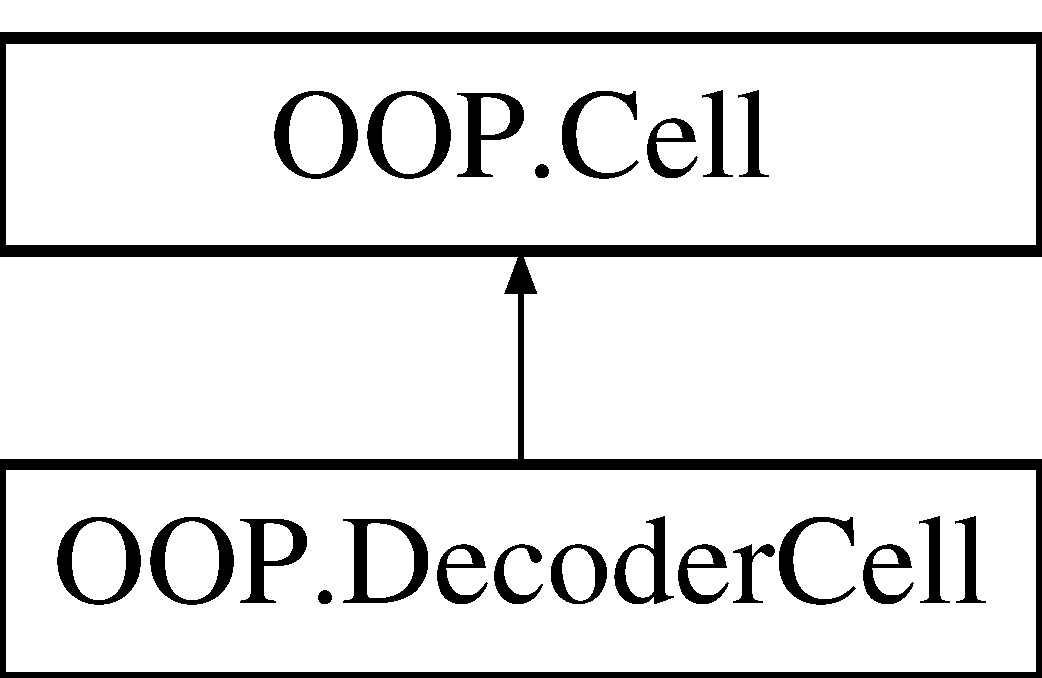
\includegraphics[height=2.000000cm]{class_o_o_p_1_1_decoder_cell}
\end{center}
\end{figure}
\subsection*{Public Member Functions}
\begin{DoxyCompactItemize}
\item 
\mbox{\Hypertarget{class_o_o_p_1_1_decoder_cell_ae361486a3a0bfd2be707a6fb6fc76222}\label{class_o_o_p_1_1_decoder_cell_ae361486a3a0bfd2be707a6fb6fc76222}} 
def {\bfseries binding} (self, encoder\+Cell)
\item 
\mbox{\Hypertarget{class_o_o_p_1_1_decoder_cell_a08d8eafb492ffde3dc5d461997faf206}\label{class_o_o_p_1_1_decoder_cell_a08d8eafb492ffde3dc5d461997faf206}} 
def {\bfseries get\+All\+Lectins} (self)
\item 
\mbox{\Hypertarget{class_o_o_p_1_1_decoder_cell_a8c5a2b96eb3d7fda5ec0ae2e6b3bb3e3}\label{class_o_o_p_1_1_decoder_cell_a8c5a2b96eb3d7fda5ec0ae2e6b3bb3e3}} 
def {\bfseries show\+Density} (self)
\item 
\mbox{\Hypertarget{class_o_o_p_1_1_decoder_cell_af8a8eee539e3b3c83f5d7ea550a5eb21}\label{class_o_o_p_1_1_decoder_cell_af8a8eee539e3b3c83f5d7ea550a5eb21}} 
def {\bfseries cytokine\+Expression} (self)
\end{DoxyCompactItemize}


The documentation for this class was generated from the following file\+:\begin{DoxyCompactItemize}
\item 
O\+O\+P.\+py\end{DoxyCompactItemize}

\hypertarget{class_o_o_p_1_1_glycan}{}\section{O\+O\+P.\+Glycan Class Reference}
\label{class_o_o_p_1_1_glycan}\index{O\+O\+P.\+Glycan@{O\+O\+P.\+Glycan}}


The documentation for this class was generated from the following file\+:\begin{DoxyCompactItemize}
\item 
O\+O\+P.\+py\end{DoxyCompactItemize}

\hypertarget{class_o_o_p_1_1_lectin}{}\section{O\+O\+P.\+Lectin Class Reference}
\label{class_o_o_p_1_1_lectin}\index{O\+O\+P.\+Lectin@{O\+O\+P.\+Lectin}}


The documentation for this class was generated from the following file\+:\begin{DoxyCompactItemize}
\item 
O\+O\+P.\+py\end{DoxyCompactItemize}

\hypertarget{class_o_o_p_1_1_simulation}{}\section{O\+O\+P.\+Simulation Class Reference}
\label{class_o_o_p_1_1_simulation}\index{O\+O\+P.\+Simulation@{O\+O\+P.\+Simulation}}


The documentation for this class was generated from the following file\+:\begin{DoxyCompactItemize}
\item 
O\+O\+P.\+py\end{DoxyCompactItemize}

\hypertarget{class_o_o_p_1_1_sphere}{}\section{O\+O\+P.\+Sphere Class Reference}
\label{class_o_o_p_1_1_sphere}\index{O\+O\+P.\+Sphere@{O\+O\+P.\+Sphere}}


Description of class \mbox{\hyperlink{class_o_o_p_1_1_sphere}{Sphere}}.  


Inheritance diagram for O\+O\+P.\+Sphere\+:\begin{figure}[H]
\begin{center}
\leavevmode
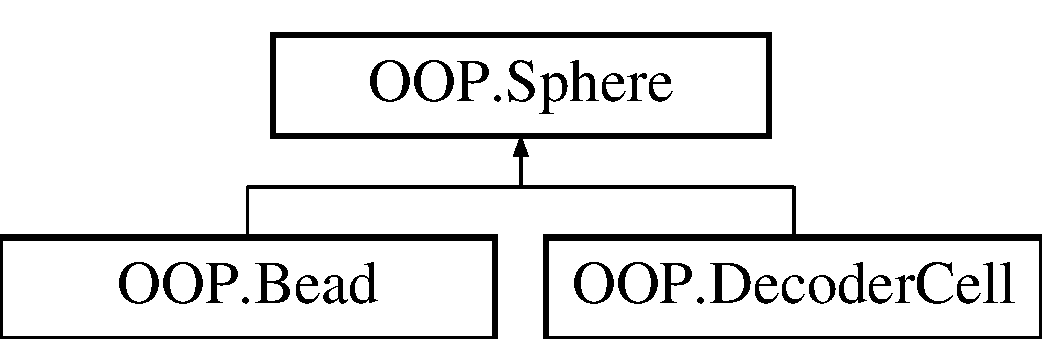
\includegraphics[height=2.000000cm]{class_o_o_p_1_1_sphere}
\end{center}
\end{figure}
\subsection*{Public Member Functions}
\begin{DoxyCompactItemize}
\item 
\mbox{\Hypertarget{class_o_o_p_1_1_sphere_a3f45e72c60b658da5354ed89fe552e7c}\label{class_o_o_p_1_1_sphere_a3f45e72c60b658da5354ed89fe552e7c}} 
def {\bfseries \+\_\+\+\_\+init\+\_\+\+\_\+} (self, I\+D\+\_\+string)
\end{DoxyCompactItemize}
\subsection*{Public Attributes}
\begin{DoxyCompactItemize}
\item 
\mbox{\Hypertarget{class_o_o_p_1_1_sphere_af3d45ee63da13a194f9ac1403b4f6809}\label{class_o_o_p_1_1_sphere_af3d45ee63da13a194f9ac1403b4f6809}} 
{\bfseries ID}
\item 
\mbox{\Hypertarget{class_o_o_p_1_1_sphere_a9645d2ffa63285cba9e349944438bc3f}\label{class_o_o_p_1_1_sphere_a9645d2ffa63285cba9e349944438bc3f}} 
{\bfseries coordinates}
\end{DoxyCompactItemize}


\subsection{Detailed Description}
Description of class \mbox{\hyperlink{class_o_o_p_1_1_sphere}{Sphere}}. 


\begin{DoxyParams}[1]{Parameters}
\mbox{\tt in}  & {\em ID} & Identifier \\
\hline
 & {\em coordinates} & Empty. Will be filled when added to \mbox{\hyperlink{class_o_o_p_1_1_well}{Well}}. \\
\hline
\end{DoxyParams}


The documentation for this class was generated from the following file\+:\begin{DoxyCompactItemize}
\item 
O\+O\+P.\+py\end{DoxyCompactItemize}

\hypertarget{class_o_o_p_1_1_well}{}\section{O\+O\+P.\+Well Class Reference}
\label{class_o_o_p_1_1_well}\index{O\+O\+P.\+Well@{O\+O\+P.\+Well}}
\subsection*{Public Member Functions}
\begin{DoxyCompactItemize}
\item 
\mbox{\Hypertarget{class_o_o_p_1_1_well_a360c562719df1b228ddafc6819678f87}\label{class_o_o_p_1_1_well_a360c562719df1b228ddafc6819678f87}} 
def {\bfseries \+\_\+\+\_\+init\+\_\+\+\_\+} (self, x, y, z)
\item 
\mbox{\Hypertarget{class_o_o_p_1_1_well_a789cba9c9e1948633d58b0c49f162b06}\label{class_o_o_p_1_1_well_a789cba9c9e1948633d58b0c49f162b06}} 
def {\bfseries border\+Control} (self, coordinates, dx, dy, dz)
\item 
\mbox{\Hypertarget{class_o_o_p_1_1_well_af0c52742fe74e6d7472730de97533164}\label{class_o_o_p_1_1_well_af0c52742fe74e6d7472730de97533164}} 
def {\bfseries add\+Bead} (self, bead, glyan\+\_\+name\+\_\+string, glycan\+\_\+type\+\_\+string, density\+\_\+percentage)
\item 
\mbox{\Hypertarget{class_o_o_p_1_1_well_aaeea044ae7dd98ef5dfcee8d9b196449}\label{class_o_o_p_1_1_well_aaeea044ae7dd98ef5dfcee8d9b196449}} 
def {\bfseries add\+Decoder\+Cell} (self, decoder\+Cell, lectin\+\_\+name\+\_\+string, lectin\+\_\+type\+\_\+string)
\end{DoxyCompactItemize}
\subsection*{Public Attributes}
\begin{DoxyCompactItemize}
\item 
\mbox{\Hypertarget{class_o_o_p_1_1_well_aac8afc46bb7b6c338653c967371f57f7}\label{class_o_o_p_1_1_well_aac8afc46bb7b6c338653c967371f57f7}} 
{\bfseries size}
\item 
\mbox{\Hypertarget{class_o_o_p_1_1_well_a12c52294dba829502ef3b3e8765010d8}\label{class_o_o_p_1_1_well_a12c52294dba829502ef3b3e8765010d8}} 
{\bfseries beads}
\item 
\mbox{\Hypertarget{class_o_o_p_1_1_well_a5911c7535990ded47917e84c165b4760}\label{class_o_o_p_1_1_well_a5911c7535990ded47917e84c165b4760}} 
{\bfseries decoder\+Cells}
\end{DoxyCompactItemize}


The documentation for this class was generated from the following file\+:\begin{DoxyCompactItemize}
\item 
O\+O\+P.\+py\end{DoxyCompactItemize}

%--- End generated contents ---

% Index
\backmatter
\newpage
\phantomsection
\clearemptydoublepage
\addcontentsline{toc}{chapter}{Index}
\printindex

\end{document}
